
\begin{figure}[h]
\centering
\scalebox{.8}
{
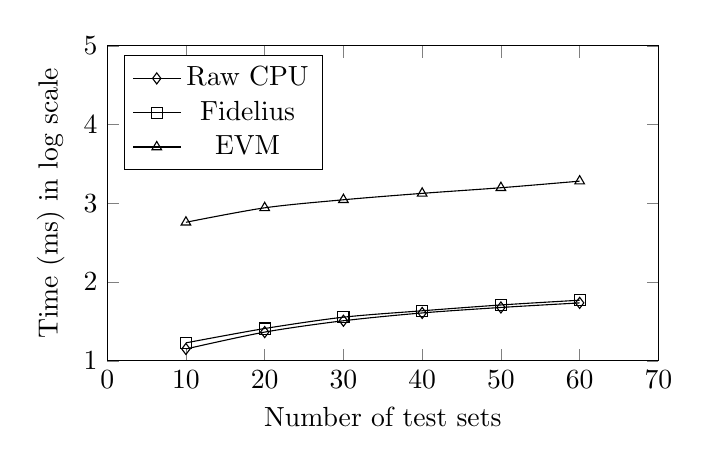
\begin{tikzpicture}
    
\pgfplotsset{
    scale only axis,
    xmin=0, xmax=70,
    ymin=1, ymax=5,
    compat=newest,
    legend pos=north west,
}

\begin{axis}[
  %axis y line*=left,
  %scaled y ticks=base 10:2,
  x=0.1cm,
  y=1cm,
  xlabel=Number of test sets,
  %width=0.4\textwidth,
  %height=0.6\textwidth,
  ylabel=Time (ms) in log scale,
]

\addplot[smooth,mark=diamond]
  coordinates{
    (10,1.1501) %log10(14.13)
    (20,1.3642) %log10(23.13)
    (30,1.5083) %log10(32.23)
    (40,1.6076) %log10(40.51)
    (50,1.6771) %log10(47.54)
    (60,1.7350) %log10(54.32)
}; \addlegendentry{Raw CPU}

\addplot[smooth,mark=square]
  coordinates{
    (10,1.2276) %log10(16.89)
    (20,1.4096) %log10(25.68)
    (30,1.5535) %log10(35.77)
    (40,1.6350) %log10(43.15)
    (50,1.7088) %log10(51.14)
    (60,1.7693) %log10(58.79)
  }; \addlegendentry{Fidelius}

\addplot[smooth,mark=triangle]
  coordinates{
    (10,2.7589) %log10(574)
    (20,2.9425) %log10(876)
    (30,3.0449) %log10(1109)
    (40,3.1261) %log10(1337)
    (50,3.1976) %log10(1576)
    (60,3.2813) %log10(1911)
  }; \addlegendentry{EVM}

\end{axis}
\end{tikzpicture}
}
  

  \caption{\small Time Consumption on Raw CPU, Fidelius and EVM.}
\label{fig:knn_cmp}
\end{figure}
